\begin{figure}[H]
\centering
\usetikzlibrary{positioning, fit, calc}   
  
\tikzset{block/.style={draw, thick, text width=2.5cm ,minimum height=1.1cm, align=center},   
line/.style={-latex}     
}  
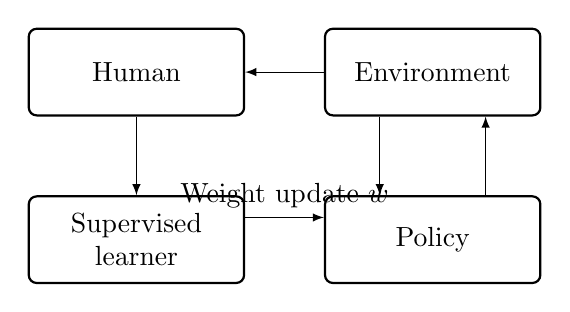
\begin{tikzpicture}  
\node[block, rounded corners=0.1cm] (human) {Human};  
\node[block,right=of human, rounded corners=0.1cm] (env) {Environment};   
\node[block, below=of env, rounded corners=0.1cm] (policy) {Policy}; 

\node[block, below=of human, rounded corners=0.1cm] (sup) {Supervised learner};  

 \draw[line] (env)-- (human);  
 %\draw[line] (policy)-- (env);  
% \draw[line] (env)-- (policy);  
 %\draw[->] (policy.140) -- (env.220);
 %\draw[->] (env.60) -- (policy.300);
 
 %\draw[red, very thick] (env.80)-- ++(1.3cm,1.3cm);
 \draw[line](env.220) -- (policy.140);
\draw[line](policy.40) -- (env.320);
\draw[line] ($(sup.north east)!0.25!(sup.south east)$) -- node[above] {Weight update $w$} ($(policy.north west)!0.25!(policy.south west)$);
 \draw[line](human.south) -- (sup.north);
    
\end{tikzpicture}  
\caption{Autoencoder, \cite{Autoencoder-tikz}} \label{fig:autoencoder}
\end{figure}



\begin{figure}[H]
\centering
\begin{tikzpicture}
  [block/.style={draw,minimum width=#1,minimum height=2em},
  block/.default=10em,high/.style={minimum height=3em},auto,
  node distance=5mm]
  %node distance=5em,auto]
  % Nodes
  \node[block=3cm,high] (n0) {Input};
  \node[block=3cm,high,right=1cm of n0] (env) {Environment};
  \node[block=3cm,high,below=of env] (policy) {Policy};
  \node[block=3cm,high,right=of policy] (PSL) {Policy Supervise Learner};
  \node[block=3cm,high,right=of policy] (HM) {Human Model};
  \node[right=1cm of PSL,align=center] (n4) {Measurement\\File};
  
  
  \draw[double,double distance=3pt,{<[policy]}-{>[US]},bend left](A)to(B){};
  \draw[double,double distance=3pt,{<[UK]}-{>[UK]},bend left](B)to(A){};

\end{tikzpicture}
\caption{Autoencoder, \cite{Autoencoder-tikz}} \label{fig:autoencoder}
\end{figure}